
\begin{figure}[H]
  \centering
  % \resizebox {\textwidth} {!} {
    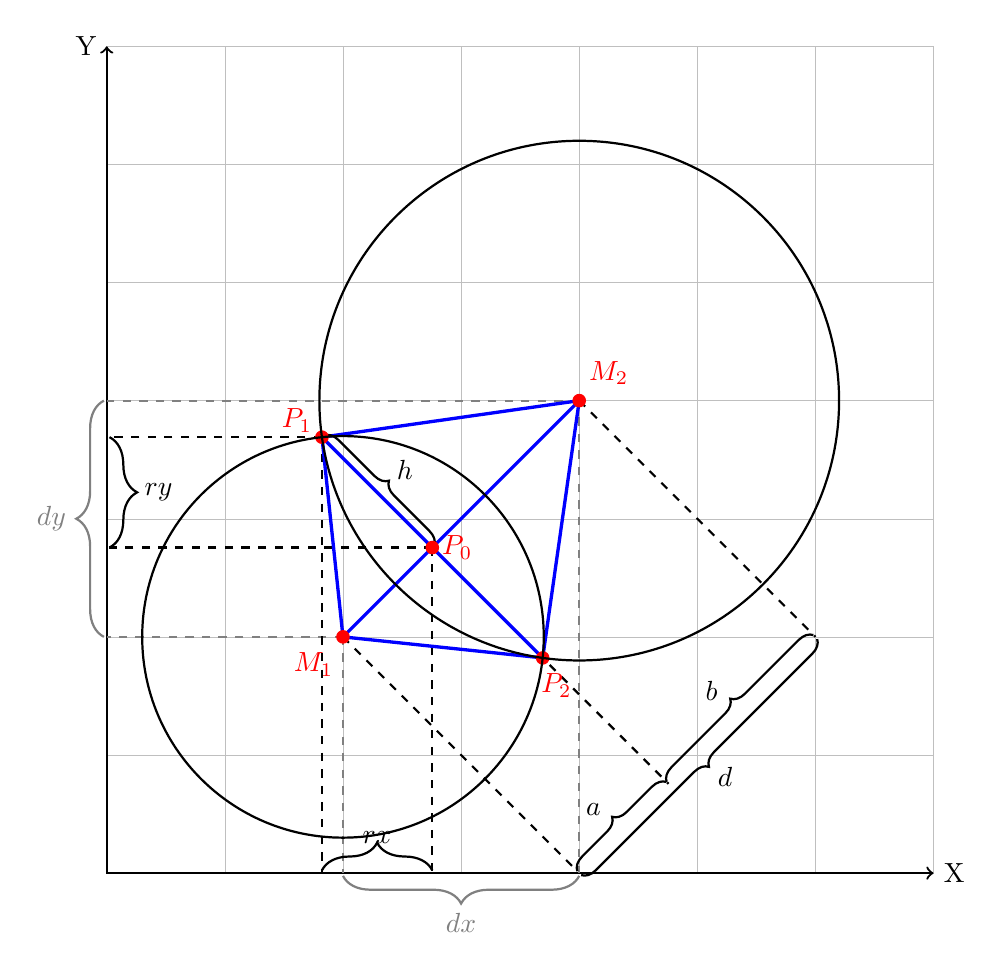
\begin{tikzpicture}[scale=1.5]
      
      % grid
      \draw[very thin,color=lightgray] (0,0) grid (7,7);
      \draw [<->,thick] (0,7) node (yaxis) [left] {Y} |- (7,0) node (xaxis) [right] {X};

      % radius of the circles
      \pgfmathsetlengthmacro{\radiusA}{1.7cm}
      \pgfmathsetlengthmacro{\radiusB}{2.2cm}
      
      % positions of circles and points
      \coordinate (A) at (2, 2);
      \coordinate (AX) at (2, 0);
      \coordinate (AY) at (0, 2);
      \coordinate (AZ) at (4, 0);
      \coordinate (B) at (4, 4);
      \coordinate (BX) at (4, 0);
      \coordinate (BY) at (0, 4);
      \coordinate (BZ) at (6, 2);
      \coordinate (C) at (2.75625, 2.75625);
      \coordinate (CX) at (2.75625, 0);
      \coordinate (CY) at (0, 2.75625);
      \coordinate (CZ) at (4.75625, 0.75625);
      \coordinate (D) at (1.8218593228739925,3.690640677126009);
      \coordinate (DX) at (1.8218593228739925,0);
      \coordinate (DY) at (0,3.690640677126009);
      \coordinate (E) at (3.690640677126009, 1.8218593228739917);
      
      % connect the positions
      \draw[thick,dashed,color=gray] (A) -- (AX);
      \draw[thick,dashed,color=gray] (A) -- (AY);
      \draw[thick,dashed] (A) -- (AZ);
      \draw[thick,dashed,color=gray] (B) -- (BX);
      \draw[thick,dashed,color=gray] (B) -- (BY);
      \draw[thick,dashed] (B) -- (BZ);
      \draw[thick,dashed] (C) -- (CX);
      \draw[thick,dashed] (C) -- (CY);
      \draw[thick,dashed] (C) -- (CZ);
      \draw[thick,dashed] (D) -- (DX);
      \draw[thick,dashed] (D) -- (DY);
      \draw[very thick,color=blue] (A) -- (B);
      \draw[very thick,color=blue] (A) -- (D);
      \draw[very thick,color=blue] (A) -- (E);
      \draw[very thick,color=blue] (B) -- (D);
      \draw[very thick,color=blue] (B) -- (E);
      \draw[very thick,color=blue] (D) -- (E);
      
      % curly braces
      \draw[thick,color=gray,decorate,decoration={brace,amplitude=10pt,mirror,raise=1pt}] (AX) -- (BX) node[midway,yshift=-18pt] {$dx$};
      \draw[thick,color=gray,decorate,decoration={brace,amplitude=10pt,raise=1pt}] (AY) -- (BY) node[midway,xshift=-20pt] {$dy$};
      \draw[thick,decorate,decoration={brace,amplitude=10pt,mirror,raise=1pt}] (CX) -- (DX) node[midway,above,yshift=7pt] {$rx$};
      \draw[thick,decorate,decoration={brace,amplitude=10pt,mirror,raise=1pt}] (CY) -- (DY) node[midway,right,xshift=10pt] {$ry$};
      \draw[thick,decorate,decoration={brace,amplitude=5pt,mirror,raise=1pt}] (AZ) -- (BZ) node[midway,xshift=10pt,yshift=-8pt] {$d$};
      \draw[thick,decorate,decoration={brace,amplitude=5pt,raise=1pt}] (AZ) -- (CZ) node[midway,xshift=-11pt,yshift=7pt] {$a$};
      \draw[thick,decorate,decoration={brace,amplitude=5pt,raise=1pt}] (CZ) -- (BZ) node[midway,xshift=-11pt,yshift=7pt] {$b$};
      \draw[thick,decorate,decoration={brace,amplitude=5pt,mirror,raise=1pt}] (C) -- (D) node[midway,xshift=10pt,yshift=8pt] {$h$};
      
      % mark the positions
      \draw[fill,color=red] (A) circle (1.5pt) node[left, yshift=-10pt] {$M_1$};
      \draw[fill,color=red] (B) circle (1.5pt) node[right, yshift=10pt] {$M_2$};
      \draw[fill,color=red] (C) circle (1.5pt) node[right] {$P_0$};
      \draw[fill,color=red] (D) circle (1.5pt) node[left, yshift=6pt] {$P_1$};
      \draw[fill,color=red] (E) circle (1.5pt) node[right, yshift=-10pt, xshift=-4pt] {$P_2$};
      
      % draw the circles
      \draw[thick,color=black] (A) circle (\radiusA);
      \draw[thick,color=black] (B) circle (\radiusB);
    \end{tikzpicture}
  % }
  \caption{Illustratie bij de methode voor het vinden van snijpunten tussen twee cirkels}
  \label{fig:snijpunten}
\end{figure}


\begin{figure}[!b]
  \centering
  \resizebox {\textwidth} {!} {
    \begin{tikzpicture}[scale=1.5]
      % grid
      \draw[very thin,color=lightgray] (0,0) grid (7,7);
      \draw [<->,thick] (0,7) node (yaxis) [left] {Y} |- (7,0) node (xaxis) [right] {X};
      
      
      \circle[1,2,1.5,1]
      \circle[2,4.5,2,1]    
      \circle[3,5.5,3,1]
      \circle[4,5,5.5,1]

      
    \end{tikzpicture}
  }
  \label{fig:voorbeeld_opgave}
  \caption{Het voorbeeld uit de opgave}
\end{figure}

\begin{figure}[H]
  \centering
  \resizebox {\textwidth} {!} {
    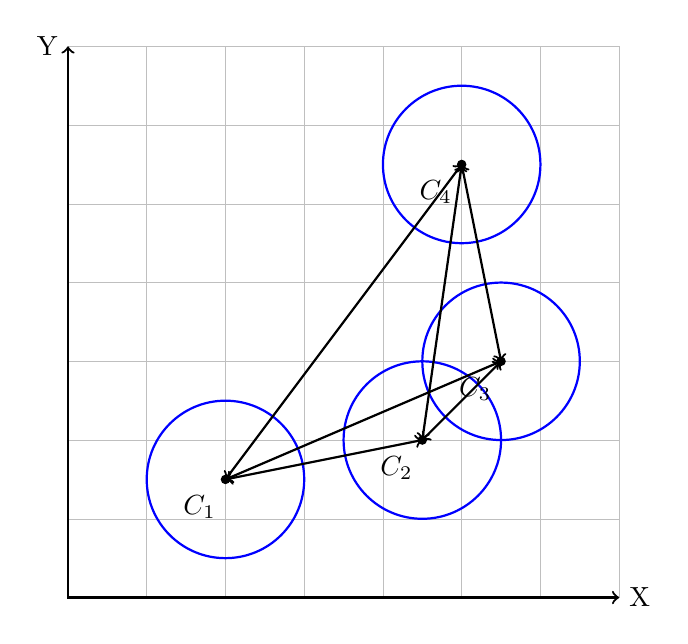
\begin{tikzpicture}[scale=1]
      % grid
      \draw[very thin,color=lightgray] (0,0) grid (7,7);
      \draw [<->,thick] (0,7) node (yaxis) [left] {Y} |- (7,0) node (xaxis) [right] {X};
      
      % Index, x, y, r
      \def\circle[#1,#2,#3,#4] {
    	% The middlepoint
    	\coordinate (C#1) at (#2,#3);
    	
    	% The point
        \draw[fill,color=black] (C#1) circle (1.5pt) node[left, yshift=-10pt, color=black] {$C_#1$};
        
        % The circle
        \draw[thick,color=blue] (C#1) circle (#4);

      }
      
      \circle[1,2,1.5,1]
      \circle[2,4.5,2,1]    
      \circle[3,5.5,3,1]
      \circle[4,5,5.5,1]
      

      \draw[thick,<->] (C1) -- (C2);
      \draw[thick,<->] (C1) -- (C3);
      \draw[thick,<->] (C1) -- (C4);
      \draw[thick,<->] (C2) -- (C3);
      \draw[thick,<->] (C2) -- (C4);
      \draw[thick,<->] (C3) -- (C4);

      
    \end{tikzpicture}
  }
  \label{fig:voorbeeld_1}
  \caption{Nagekeken cirkels bij algoritme 1}
\end{figure}
\begin{figure}[!b]
  \centering
  \resizebox {\textwidth} {!} {
    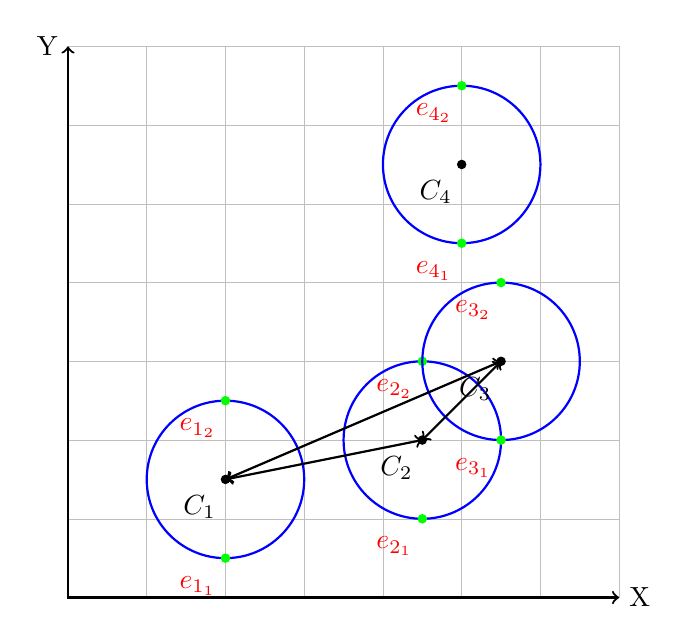
\begin{tikzpicture}[scale=1]
      % grid
      \draw[very thin,color=lightgray] (0,0) grid (7,7);
      \draw [<->,thick] (0,7) node (yaxis) [left] {Y} |- (7,0) node (xaxis) [right] {X};
      
      % Index, x, y, r
      \def\circle[#1,#2,#3,#4] {
    	% The middlepoint
    	\coordinate (C#1) at (#2,#3);
    	
    	
    	% The point
        \draw[fill,color=black] (C#1) circle (1.5pt) node[left, yshift=-10pt, color=black] {$C_#1$};
        
        % The circle
        \draw[thick,color=blue] (C#1) circle (#4);		
        
        % The eventpoints
        \coordinate (E#1_1) at (#2,#3-#4);
        \coordinate (E#1_2) at (#2,#3+#4);
    	
        \draw[fill, color=green] (E#1_1) circle (1.5pt) node[left, yshift=-10pt, color=red] {$e_{#1_1}$};
        \draw[fill, color=green] (E#1_2) circle (1.5pt) node[left, yshift=-10pt, color=red] {$e_{#1_2}$};
      }
      
      \circle[1,2,1.5,1]
      \circle[2,4.5,2,1]    
      \circle[3,5.5,3,1]
      \circle[4,5,5.5,1]
      

      \draw[thick,<->] (C1) -- (C2);
      \draw[thick,<->] (C1) -- (C3);
      \draw[thick,<->] (C2) -- (C3);


      
    \end{tikzpicture}
  }
  \label{fig:voorbeeld_2}
  \caption{Nagekeken cirkels bij algoritme 2}
\end{figure}
\begin{figure}[H]
  \centering
  % \resizebox {\textwidth} {!} {
    \begin{tikzpicture}[scale=1]
      % grid
      \draw[very thin,color=lightgray] (0,0) grid (7,7);
      \draw [<->,thick] (0,7) node (yaxis) [left] {Y} |- (7,0) node (xaxis) [right] {X};
      
      \indexedcircle[1,2,1.5,1]
      \indexedcircle[2,4.5,2,1]    
      \indexedcircle[3,5.5,3,1]
      \indexedcircle[4,5,5.5,1]

      \draw[thick,color=blue,arrows={Triangle[scale=1]-Triangle[scale=1]}] (C2) -- (C3);


      
    \end{tikzpicture}
  % }
  \label{fig:voorbeeld_23}
  \caption{Nagekeken cirkels bij algoritme 3}
\end{figure}

\begin{figure}[H]
   \centering
   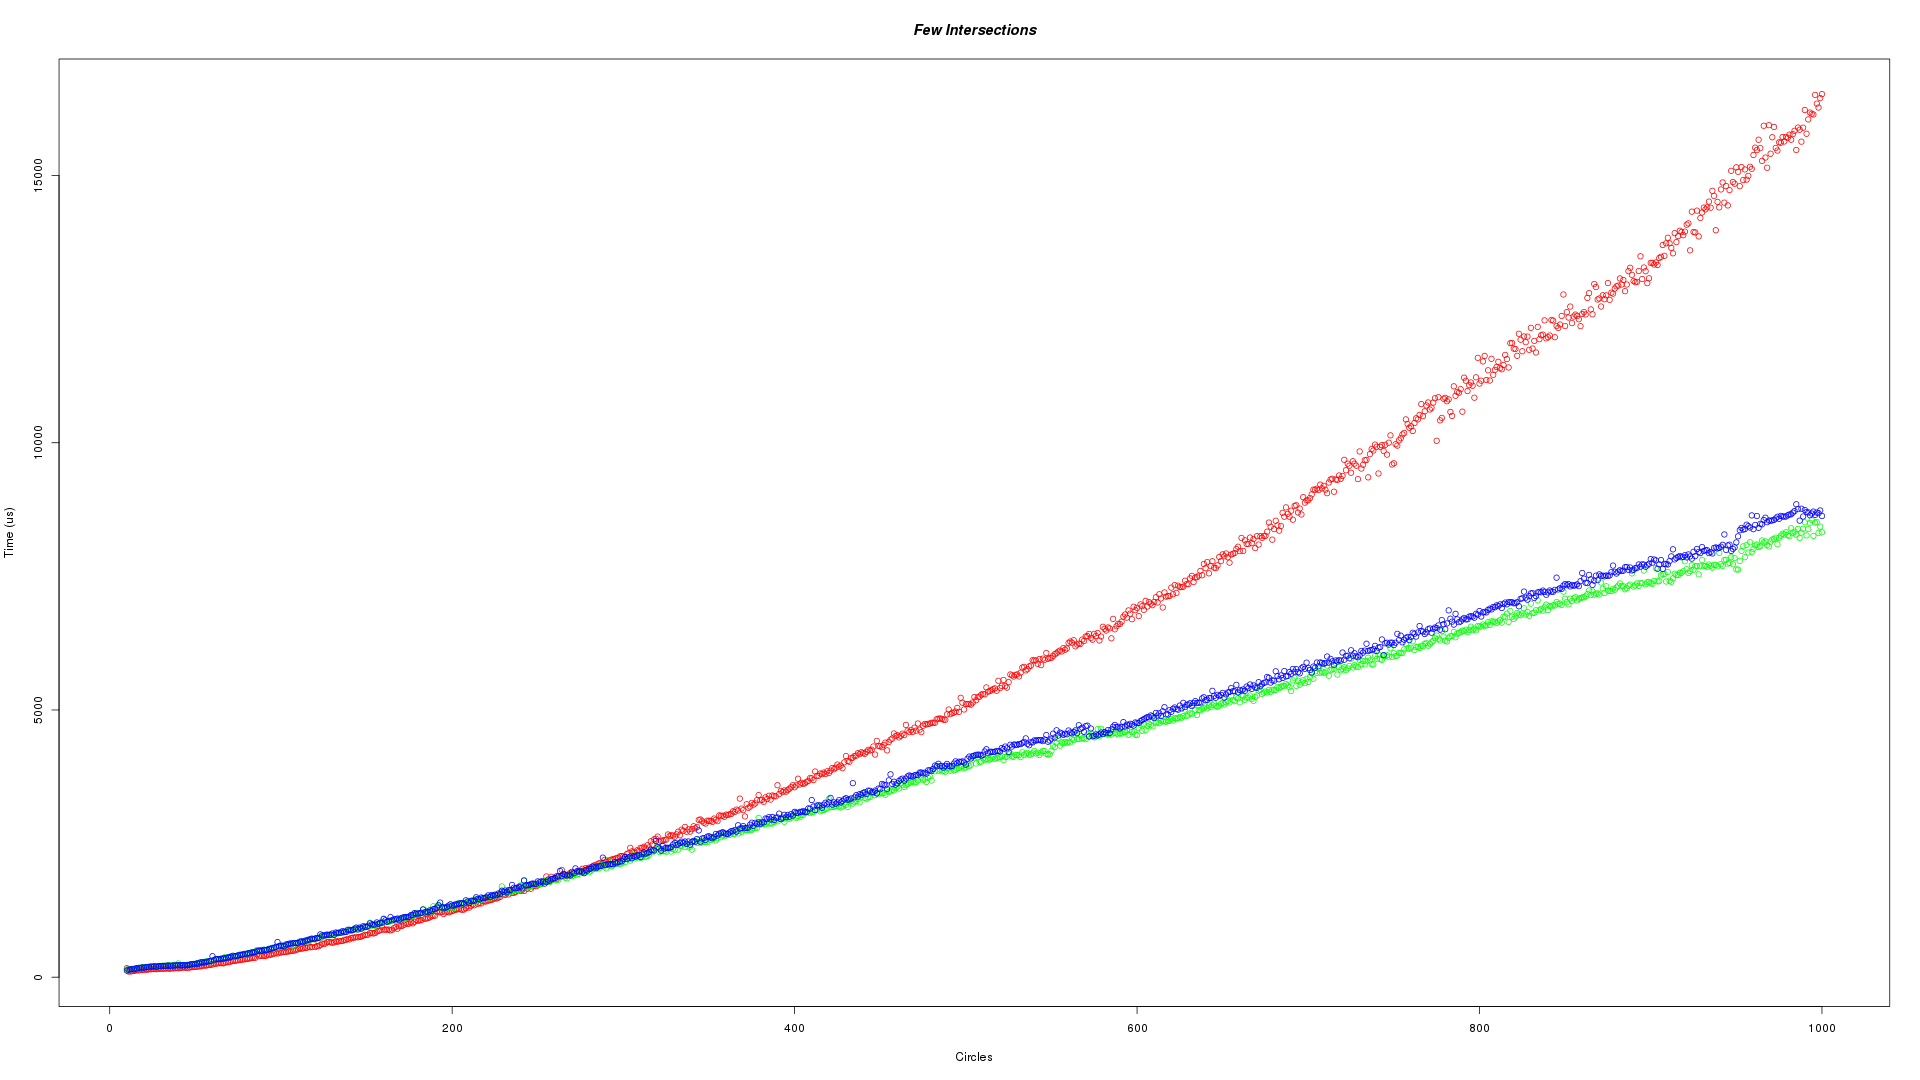
\includegraphics[width=1\textwidth]{illustraties/fewIntersections.png}
\end{figure}
   
\begin{figure}[H]
   \centering
   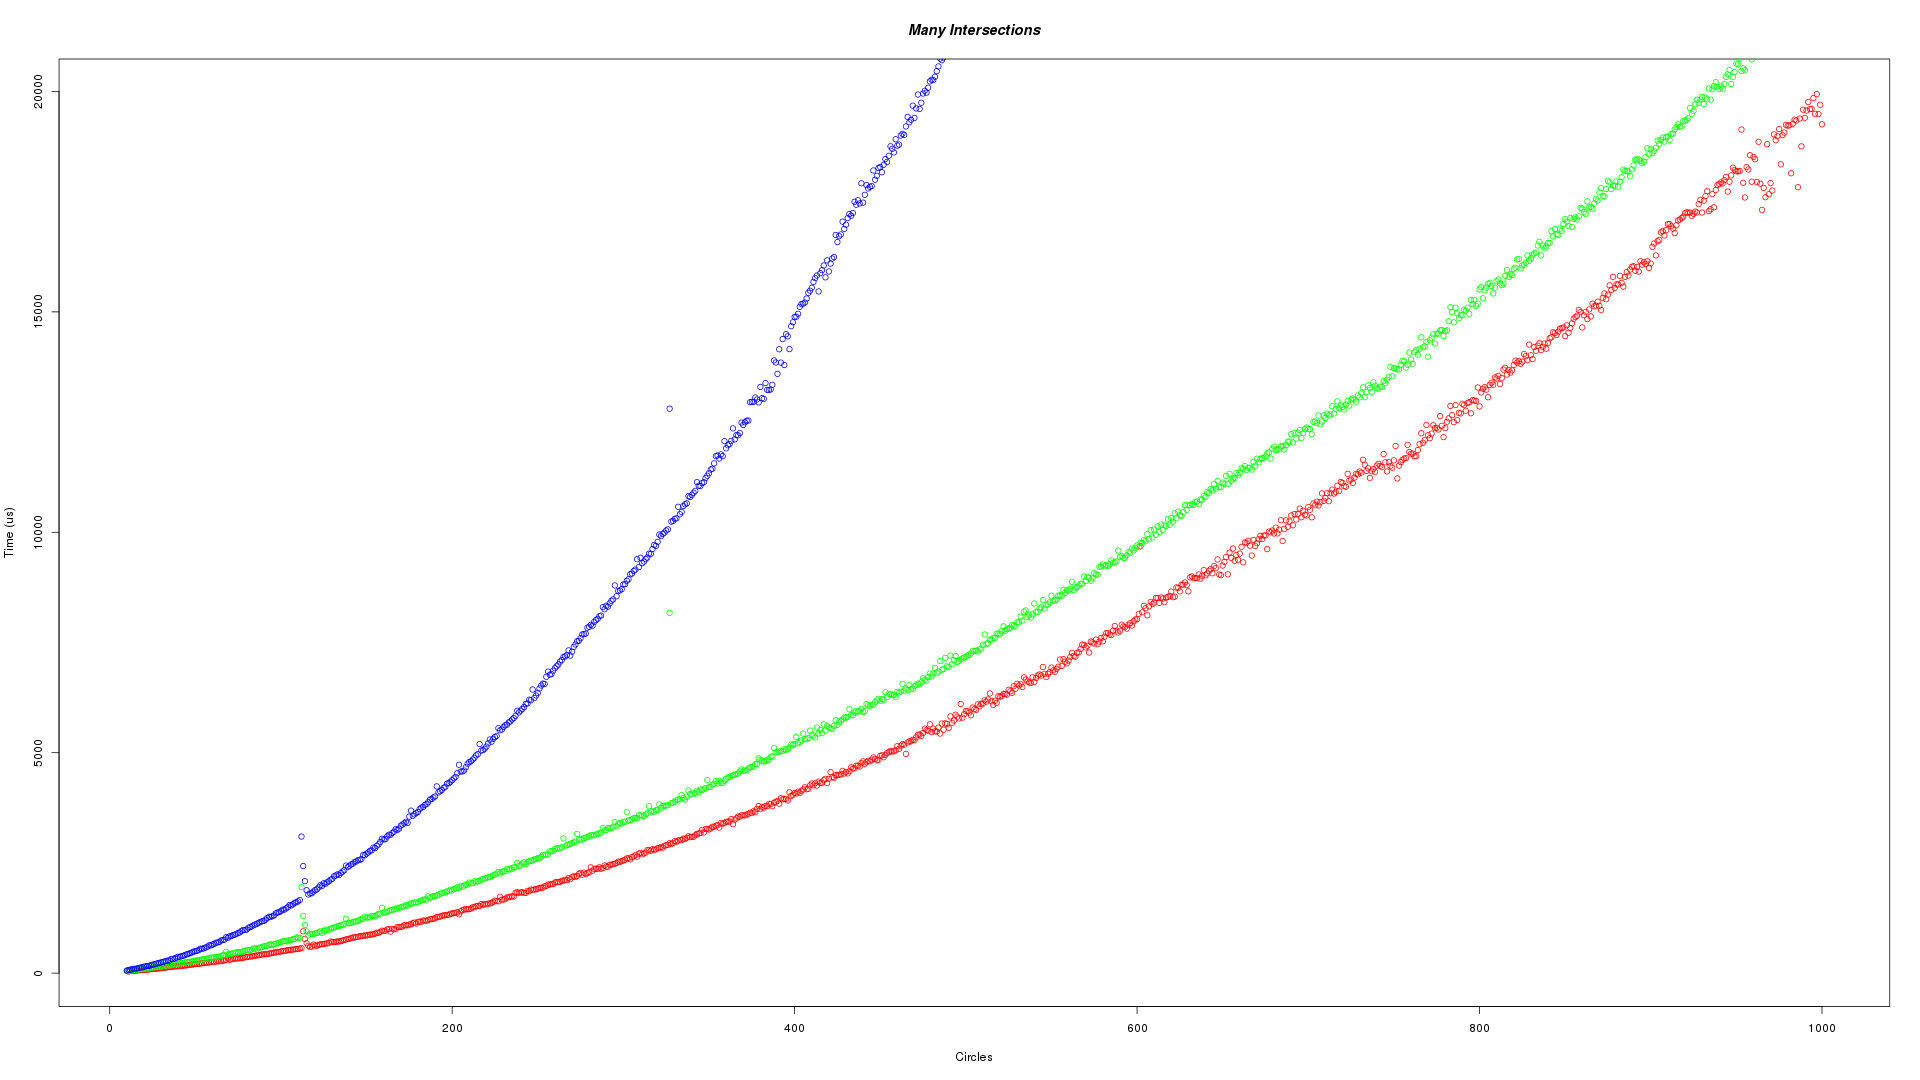
\includegraphics[width=1\textwidth]{illustraties/manyIntersections.png}
\end{figure}

\begin{figure}[H]
   \centering
   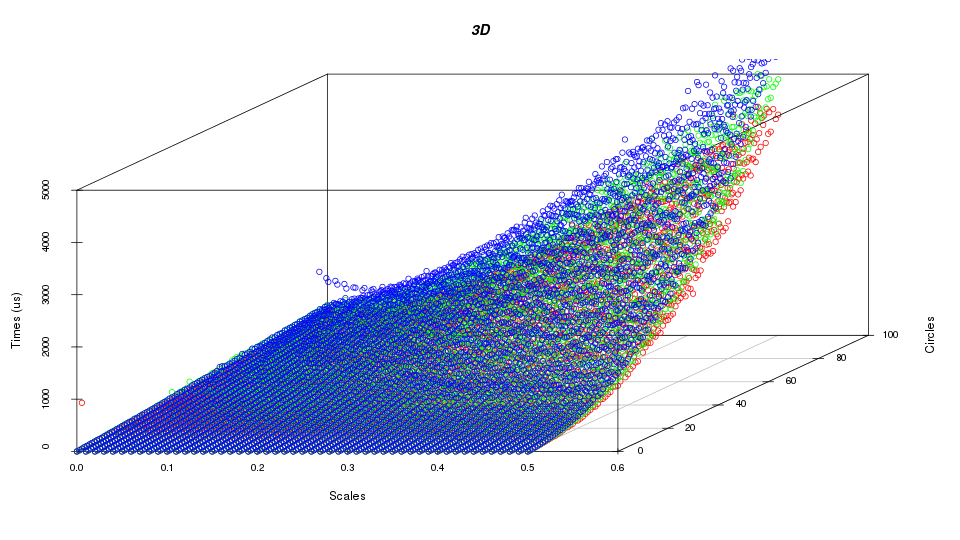
\includegraphics[width=1\textwidth]{illustraties/3DScatter.png}
\end{figure}

\begin{figure}[H]
   \centering
   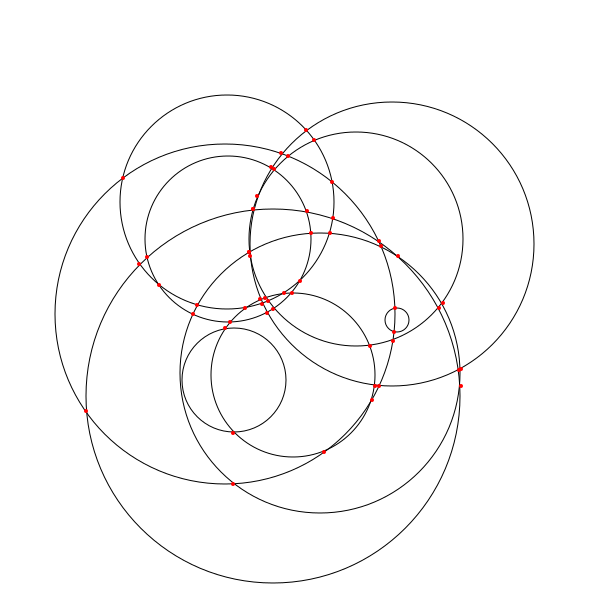
\includegraphics[width=1\textwidth]{illustraties/visuele_output.png}
\end{figure}

\subsection{Doubling Ratio}

\begin{figure}[H]
\[
\begin{array}{|c||ccccccc|}
\hline 
& 20 & 40 & 80 & 160 & 320 & 640 & 1280\\
\hline \hline 
0.000 & 3.4 & 3.9 & 4.6 & 4.2 & 4.3 & 4.3 & 4.2 \\ \hline 
0.001 & 3.2 & 4.3 & 4.2 & 4.9 & 4.1 & 4.3 & 4.2 \\ \hline 
0.500 & 3.5 & 4.0 & 4.5 & 4.8 & 4.9 & 4.8 & 5.0 \\ \hline 
1.000 & 3.4 & 4.2 & 4.5 & 4.7 & 5.3 & 5.3 & 5.3 \\ \hline 
\end{array}
\]


\label{doublingratio_1}
\caption{Doubling ratio 1}
\end{figure}
tekst
\begin{figure}[H]
\[
\begin{array}{|c||ccccccc|}
\hline 
& 20 & 40 & 80 & 160 & 320 & 640 & 1280\\
\hline \hline 
0.000 & 1.8 & 2.3 & 2.2 & 2.3 & 2.1 & 2.2 & 2.1 \\ \hline 
0.001 & 2.0 & 2.4 & 2.1 & 2.5 & 2.2 & 2.3 & 2.6 \\ \hline 
0.500 & 3.1 & 3.9 & 4.2 & 4.3 & 5.1 & 5.2 & 5.1 \\ \hline 
1.000 & 3.7 & 4.3 & 4.0 & 4.7 & 5.5 & 5.1 & 5.4 \\ \hline 
\end{array}
\]


\label{doublingratio_2}
\caption{Doubling ratio 2}
\end{figure}

\begin{figure}[h]
\[
\begin{array}{|c||ccccccc|}
\hline 
& 20 & 40 & 80 & 160 & 320 & 640 & 1280\\
\hline \hline 
0.000 & 2.2 & 2.2 & 2.2 & 2.3 & 2.2 & 2.1 & 2.2 \\ \hline 
0.001 & 2.1 & 2.2 & 2.2 & 2.3 & 2.8 & 1.8 & 2.4 \\ \hline 
0.500 & 3.3 & 3.4 & 4.1 & 4.4 & 5.2 & 5.2 & 5.0 \\ \hline 
1.000 & 3.4 & 4.0 & 4.2 & 4.6 & 5.5 & 5.1 & 5.1 \\ \hline 
\end{array}
\]


\label{doublingratio_3}
\caption{Doubling ratio 3}
\end{figure}
